% to submit via https://www.easychair.org/account/signin.cgi?conf=europar2013
% max 12 pages
\documentclass{llncs}
%
\usepackage{listings}
\usepackage{url}
\usepackage{todo}
\usepackage{xcolor}
\newcommand\see{\emph{cf.\ }}

\usepackage{tikz}
\usetikzlibrary{positioning}
\usetikzlibrary{shadows}
\usetikzlibrary{arrows}
\usetikzlibrary{shapes}


\lstset{language=python,morekeywords={cimport, cdef, with},
basicstyle=\ttfamily, keywordstyle=\bf, stringstyle=\color{gray}}

\begin{document}
% update listing numbering
\renewcommand{\thelstlisting}{\arabic{lstlisting}}
%
\title{Pythran: Bringing OpenMP to a Python Subset}

\author{Serge Guelton\inst{1,2} \and Pierrick Brunet\inst{2}}

\institute{
    {\'E}cole Normale Sup{\'e}rieure, Paris, France
    \and
    T{\'e}l{\'e}com Bretagne, Plouzan{\'e}, France
}

\maketitle

\marginpar{The title is to be changed}
%
\begin{abstract}

    The Python language offers an interesting solution as a scientific
    computing language thanks to the SciPy package. However, the lack of
    fine-grained parallelism support remains an important shortcoming. This
    paper proposes to add OpenMP directives to the Python language and shows
    that it is possible to turn a module written in a large Python subset
    enhanced with these directives into a native parallel module that runs as
    fast as its naive C equivalent, while keeping the input code totally
    compatible with the python interpreter. The approach is validated through
    the Pythran compiler.

\keywords{Python, OpenMP, C++, static compilation, scripting language.}
\end{abstract}

%
\section{Introduction}

Since its birth in December 1989, the Python language~\cite{rossum97} has proved
to be useful in various domains, ranging from system administration to web
services, thanks to its dynamicity, expressiveness, rich ecosystem and
battery-included standard library. It is also getting widely used in scientific
computing~\cite{Oliphant2007}, mainly thanks to the SciPy~\cite{scipy} project
that adds MATLAB-like functionalities to the language.

The prohibitive performance overhead of the language implied by its interpreted
and highly dynamic nature does not prevent its usage as a language for high
performance computing. SciPy overcomes this issue through low-level routines
written in C or Fortran and encapsulated in Python \emph{native} modules.
Moreover, its core data structure, the multi-dimensional
array~\cite{numpyarray2011}, has been designed so that the underlying data are
available to both native modules and the Python interpreter without conversion
cost.

To enable the user to write native functions, without having to write the glue
code that turns Python object into native structures back and forth, the SciPy
package provides the \texttt{weave} module that makes it possible to bundle C
code snippet into Python code and compile then load them at runtime.

This hybrid approach, based on a mix of interpreted and native code, is getting
widespread in the Python landscape. Section~\ref{sec:python-parallel} studies
the existing approaches and shows a critical lack of parallelism support, and
emphasises on the need for a backward-compatible approach.
Section~\ref{sec:python-openmp} studies the validity of using OpenMP directives
within the Python language in order to add fine-grain parallelism support to
Python in the context of a Python subset called Pythran. Static compilation of
this language into C++ and the underlying runtime is described in
Section~\ref{sec:python-static}. The Pythran compiler is benchmarked on several
scientific kernels and compared to Cython in Section~\ref{sec:validation}.

%=========================================================
\section{Parallel Computations in Python}\label{sec:python-parallel}
%=========================================================

In the many cores area, turning to parallelism to balance the performance
limitations of scripting languages, as described 
% in~\cite{choy05} in the context of the MATLAB language, or
in~\cite{mals07} in the context of the R language, seems legitimate. In the
context of Python, most approaches have focused on fork-based parallelism.

\subsection{Python and Parallelism}

Parallel computations are supported by the Python standard library through the
\texttt{multiprocessing} module. It spawns several interpreters that can
communicate through IPC, using Python built-in object serialization. This
approach is only viable for computation intensive application. Furthermore, the
communication and synchronization overheads are much greater than a light-weight
processes approach.

Although the standard \texttt{threading} module makes it possible to start
several light-weight threads within the same interpreter, this approach is not
relevant for HPC, because of a specificity of CPython, the \emph{Global
Interpreter Lock}~\cite{gil2012}.\footnote{Other Python interpreters, such as
IronPython or Jython, do not have a GIL.} This lock ensures that only one thread
is active at a time in the interpreter. While it makes it possible to have
cooperative threads, say for a GUI, it does not take advantage of multiple
cores.  However, there are two notable exceptions: the GIL is released on I/O,
and the GIL does not prevent the use of threads inside native modules, where the
user has full control.

To illustrate this behavior, we used the CPU-bound Buffon's needle algorithm to
estimate the value of $\pi$. Its execution time using a multi-threaded
implementation on 4 cores is $\times 1.46$ the execution time of the sequential
version. So the GIL contention actually \emph{increases} the execution time.

As a consequence, Python developers need to write multi-threaded native
modules in order to fully benefit from multiple cores. This leads to a kind of
computations referred as hybrid computations.

%There have been several approaches to replace the GIL by Transactional
%Memories~\cite{Riley2006,Tabba2010} but none of them made there way to the
%mainstream interpreters.


\subsection{Hybrid Computations}

In the context of interpreted languages, \cite{dongara2007} defines a computation
as \emph{hybrid} when part of the code is interpreted, and part of it is
executed natively.

It is now common for scripting language to have C bindings. To take advantage of
compiled code, and to overcome the GIL limitations, Python developers must write
parallel C/C++ functions and the associated boilerplate based on the Python C
API~\cite{pythoncapi}. Tools have been developed to relieve the user from
writing the encapsulating code, notably SWIG~\cite{swig2003} that relies on an
enhanced interface specification, or
\texttt{boost::python}~\cite{boostpython2007} that relies on C++ facilities to
guide translation.

An opposite approach consists in using the host language ---herein Python--- to
describe both parts of the system, and to let an automated tool perform the
translation to native code of a part of the application, generally the
computation-intensive one where parallelism has been expressed in some ways.
Thus, developers not familiar with lower level languages or not eager to invest
the additional development time can still benefit from a fair performance boost.
This approach is the subject of many studies that can be classified according to
their compatibility with the host language.

\subsubsection{Backward-Incompatible Approaches}

A constraining (from the performance point of view) aspect of the Python
language is its type system. It implies that each method call is resolved
dynamically, even a simple add operation! It comes at no surprise that many
approaches restrain the Python language to add a static typing overlay.  Also,
only two types of integers (64-bit integers and multi-precision integers) and
one type of floating point type (double-precision floats) are available in
Python, so using a type with the appropriate size may lead to significant
performance boost.

Cython~\cite{cython2010} is such a Python dialect. It extends the syntax with
typing informations, calls to native functions from third party libraries, and a
limited set of parallelism constructs, such as the possibility to define
parallel loops, but no task parallelism. PLW~\cite{dongara2007} proposes a
similar approach that mixes Python with C, using raw strings to hold the C code
and the parallel directives, that are limited to parallel for loops.
%The numba~\footnote{\emph{cf}.\ \texttt{https://github.com/numba/numba}}
%compiler uses additional type information to generate sequential LLVM bytecode.
PyCUDA and PyOpenCL~\cite{klockner2012} also target accelerators by mixing
Python with kernels embedded as raw strings containing accelerator code.

The main issue of these approaches is that they imply to modify, in a more or
less complex way, the original code. They require to learn a new dialect,
and the long-term preservation of this investment is not ensured. Moreover,
there is no falling back if the code were to be deployed in an environment
where the parallelizing tool/module is not available. For instance, once a code
has been ported to PyCUDA and transformed into CUDA code embedded in Python
strings, there is no way back and the developer has to maintain two versions of
the algorithm.

\subsubsection{Backward-Compatible Approaches}

Most backward-compatible approaches also require to modify the input program.
They do not extend the Python language, but restrict it. As a consequence, they
remain compatible with the original language and do not suffer from the
drawbacks of the previous approaches. They also benefit from existing tools
associated to the language.

Copperhead~\cite{copperhead2011} is a functional, data parallel language
embedded in Python. It uses n-uplets, numpy arrays and lists as its core data
structure and prohibits usage of many control-flow operators such as loops,
enforcing the use of the \texttt{map}, \texttt{filter} or \texttt{reduce}
intrinsics to exhibit parallelism. But it can be efficiently compiled to either
CUDA or C++ with calls to the Thrust\footnote{\emph{cf}.\
\texttt{http://thrust.github.com/}} library. Python decorators are used to
identify hot-spots that are JIT-compiled to native code.

Tools such as PyPy~\cite{pypy2009}, a Python interpreter with a tracing JIT, or
Shedskin~\cite{shedskin2006}, a Python to C++ compiler are also viable ways to
turn regular Python codes into optimized ones, but they do not offer support for
fine-grained parallelism beyond what the standard library proposes.
%~\footnote{Shedskin is compatible with several Python modules that provide
%coarse-grained, fork-based parallelism.}

To be completely backward compatible, it must be possible to run the input code
in an environment that is not aware of the existence of the parallelizing
solution. This principle is not respected by parallel libraries, but code
annotations satisfy it. This is where OpenMP~\cite{openmp3.1} parallel
annotations shine: the original code remains compatible with a compiler that is
not aware of OpenMP.

This article proposes to combine OpenMP~\cite{openmp3.1} parallel annotations
with a Python subset called Pythran to bring fine-grain parallelism to Python.
While being backward compatible with both the Python language, and the
sequential algorithm. It means that:
%
\begin{enumerate}
    \item Any Pythran code can be run (sequentially), with no module dependency
        or code change, by any Python interpreter.
    \item Parallelism is explicit and incrementally added to the original code
        through directives.
\end{enumerate}

%=========================================================
\section{OpenMP Semantical Adaptations}\label{sec:python-openmp}
%=========================================================

OpenMP is a standard API for parallel programming for Fortran, C and C++. It
consists in a set of parallelizing directives and a few runtime library calls.
If OpenMP is not activated, the directives are ignored, thus enabling
incremental parallelization of the original source code while keeping the
original code structure. The languages targeted by OpenMP are statically
compiled. This section studies the semantical adaptation required to use the
same API for a scripting language such as Python.

\subsection{Directives}

OpenMP directives are held by C/C++ pragma, or by Fortran comments. Most of them
apply to structured blocks, represented by an instruction in C/C++ and delimited
by comments in Fortran. A few directives (e.g.\ \texttt{threadprivate}) are not
attached to a specific instruction.

While Pythran has a decorator mechanism\footnote{\see PEP 318,
\url{http://www.python.org/dev/peps/pep-0318/} for a more detail explanation of
Python decorators.}, it only applies to functions, methods and classes and does
not make it possible to attach decorations to other statements. Pythran uses
the path taken by PLW~\cite{dongara2007}, that uses string instructions to hold
such decorations. As Python does not have anonymous block,
%~\footnote{\see PEP340, \url{http://www.python.org/dev/peps/pep-0340/} for a
%discussion concerning anonymous block support in Python.}
one has to create a dummy \texttt{if 1:} instruction to apply an annotation to a
whole block. Alternatively, the syntax \texttt{if 'my annotation':} is also
supported. 

%Listing~\ref{lst:instruction-annotation} shows how to annotate a
%parallel loop with reduction this way.
%
%\begin{figure}
%    \begin{lstlisting}[label={lst:instruction-annotation}, caption={Parallel
%    loop with reduction annotated with OpenMP directive.}]
%'omp parallel for reduction(+:r)'
%for auto in my_container: r += x
%  \end{lstlisting}
%\end{figure}

Many OpenMP annotations are parametrized by clauses that list variables,
specifying their behavior with respect to parallel regions, e.g.\
\texttt{private}, \texttt{shared}, \texttt{copyin}. They can only refer to
variables that have already been declared. However, there is no variable
declaration in Python, and all variables assigned in a function have the
function scope. Consequently, all variables that are referenced in a function
are considered when building such variable lists: there is no concept of
variable local to a block. Using the \texttt{default(none)} clause is possible
to ensure no variable gets forgotten when building such lists.

The \texttt{reduction(\emph{operator}: \emph{list})} directive is used to
characterize some data dependencies when performing a parallel reduction. The
list of supported operators depend on the input and backend languages: Python
has \texttt{min}/\texttt{max} operators but C/C++ does not. C/C++ have
\texttt{\&\&} or \texttt{||} while Python does not.\footnote{Although similar,
the \texttt{and} and \texttt{or} keywords have a special meaning in Python.}

\subsubsection{Parallel For and Iterators}

The core directive to handle data parallelism is the \texttt{for} directive that
distributes the iteration space of the associated loop among the existing
threads. To be compatible with OpenMP, the loop iteration space must be
described by a random access iterator with a total order. Integers used as loop
indices in Fortran and C satisfy this conditions, as well as C++ iterators with
the \texttt{random\_access\_tag} trait. But a Python iterator only advances by a
step of one until it is exhausted, in which case it raises an exception: it
behaves as a forward iterator. To be compatible with OpenMP, these iterators
must be turned into random access iterators.

The extension of Python iterator to random access iterators is direct for the
standard containers: \texttt{list}\footnote{Python \texttt{list}s behave as C++
\texttt{vector}s.}, \texttt{set} or \texttt{dict}. Other iterators require more
care.

Generators, Python objects that behave like iterators, are commonly used in
Python. The simplest one, \texttt{xrange(\emph{start}, \emph{stop},
\emph{step})}, successively yields value starting from \texttt{\emph{start}} to
\texttt{\emph{stop}} by a step of \texttt{\emph{step}}. It is easily extended to
support random access, but it generally does not make sense to use a generator
as a loop iterator, as the relation between two random states of the iterator
may be of an arbitrary complexity.

Generator expressions are generators whose content is built from an other
iterator. For instance \texttt{(x*x for x in l)} successively yields the square
of each element in \texttt{l}. They behave like adaptors: they apply a
particular expression on each value of the iterator. It is also the case of the
\texttt{enumerate} builtin, that yields each element of the enumerated iterator
associated with its index. These generators are random iterators only if their
input iterator is a random iterator itself.

Finally, if the iterator yields a tuple, it is possible to unpack it inside the
\texttt{for} construct, as shown in Listing~\ref{lst:complex-omp-for}. In that case
all the unpacked variables are considered as iterators, especially with respect
to default privatization rules: in the given example, \texttt{i} and \texttt{v}
are private, and the parallel iteration is valid because the input of
\texttt{enumerate} is a list, which allows random access iteration.

\begin{figure}
    \begin{lstlisting}[label={lst:complex-omp-for}, caption={Parallel
    loop in Pythran with tuple unpacking.}]
'omp parallel for'
for i, v in enumerate([2, 3, 5, 7, 11]): print i, ':', v
  \end{lstlisting}
\end{figure}

Pythran runtime is aware of these three kind of iterators: random access
iterators for standard containers, adaptor iterators for generator expressions
and forward iterators for generators.

\subsection{Runtime Library}

OpenMP provides a small runtime library that, for instance, makes it possible to
retrieve the active thread id. All the functions are declared in the
\texttt{<omp.h>} header, and have a default behavior when OpenMP is not
activated.

Providing a binding to these library in Python does not raise particular
problems, as the signature of these functions only involves integers passed as
parameters or return values, except for the mutex manipulation. In that case an
opaque type is used to represent the native type.

The \texttt{\_OPENMP} macro definition is always provided when OpenMP is
activated, and can be used to detect when OpenMP is not available. Python does
not have a preprocessor, but it is possible to catch the import exception if the
\texttt{omp} module is not found.

\subsection{Validation}

A validation suite for OpenMP is proposed in~\cite{wang2012} for C and Fortran.
We ported it to Python, and also extended it to validate the corner cases
specific to Python described in this section. A typical test case is given in
Listing~\ref{lst:openmp-validation}.

\begin{figure}
    \begin{lstlisting}[label={lst:openmp-validation},caption={Example of Python
    OpenMP validation test case.}]
def omp_parallel_for_if(loop_count):
  import omp
  using = sum = 0
  'omp parallel for if(using == 1)'
  for i in range(loop_count + 1):
    num_threads = omp.get_num_threads()
    sum += i
  known_sum = (loop_count * (loop_count + 1)) / 2
  return known_sum == sum and num_threads == 1
    \end{lstlisting}
\end{figure}

We have used the Pythran tool described in the following section to turn each
Python test function into a C++ function with the same directives and runtime
calls. Apart from the \texttt{threadprivate} directive and the
\texttt{collapse(\emph{n})} clause, all tests were successful.
\texttt{threadprivate} directives were held by global variables not supported in
Pythran yet~; and the C++ code generated by Pythran does not preserve the perfect
loop nesting required by the \texttt{collapse} clause.

%=========================================================
\section{Static Translation of Python Programs}\label{sec:python-static}
%=========================================================

Pythran is a subset of Python designed for scientific computing. It is
implicitly statically typed and supports most Python constructs except those
that involve introspection (e.g.\ \texttt{getattr}) or runtime compilation
(e.g.\ \texttt{eval}). A few standard modules are supported in addition to the
core language (e.g.\ \texttt{math}, \texttt{random}). The \texttt{numpy} module
is currently only partially supported. The associated compiler turns Pythran
code, possibly annotated with OpenMP and a few function type annotations, into
C++ code. Its processing is summarized in Figure~\ref{fig:pythran-compiler} and
relies on type inference to remove most dynamic behavior, combined with a
high-level runtime library, \texttt{pythonic++}, to allow a one-to-one mapping
between Python and C++ constructs. The purpose of this section is not to dig
into the internals of the compiler, but rather to focus on the impact of the
parallelism layer, especially on the runtime library.

\begin{figure}

\centering
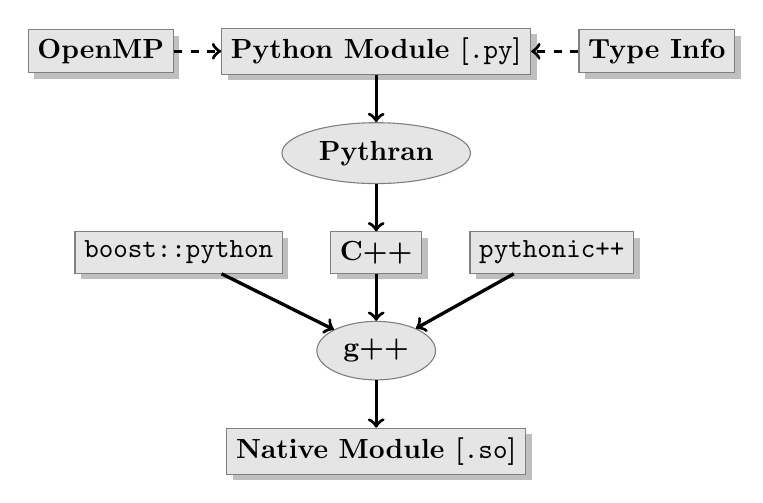
\begin{tikzpicture}[
file/.style={draw=black!50,fill=black!10,rectangle, drop shadow, align=center,
node distance=0.6cm},
    tool/.style={draw=black!50,fill=black!10,ellipse, align=center, node
distance=0.6cm}]
\node[file] (python) {\textbf{Python Module [\texttt{.py}]}};
\node[file] (annotation)	   [right=of python] {\textbf{Type Info}};
\node[file] (omp)	   [left=of python] {\textbf{OpenMP}};
\node[tool] (pythran) [below=of python] {\textbf{Pythran}};
\node[file] (cxx) [below=of pythran] {\textbf{C++}};
\node[file] (boost) [left=of cxx] {\textbf{\texttt{boost::python}}};
\node[file] (pythonic) [right=of cxx] {\textbf{\texttt{pythonic++}}};
\node[tool] (gxx) [below=of cxx] {\textbf{g++}};
\node[file] (so) [below=of gxx] {\textbf{Native Module [\texttt{.so}]}};

\draw[very thick, ->] (python) -- (pythran);
\draw[very thick,dashed, ->] (annotation) -- (python);
\draw[very thick,dashed, ->] (omp) -- (python);
\draw[very thick, ->] (pythran) -- (cxx);
\draw[very thick, ->] (cxx) -- (gxx);
\draw[very thick, ->] (boost) -- (gxx);
\draw[very thick, ->] (pythonic) -- (gxx);
\draw[very thick, ->] (gxx) -- (so);
\end{tikzpicture}
\caption{Pythran compiler workflow.}
\label{fig:pythran-compiler}
\end{figure}

\subsection{Runtime Support}

Pythran runtime is based on the STL. The standard library of C++11, unlike its
C++03 version, is thread-safe, so the data dependencies in the original code
remain explicit.

A critical point of the design of the \texttt{pythonic++} runtime is memory
management, the very same aspect that led to the use of a GIL in CPython.
Memory management is implemented in Shedskin through the general-purpose Boehm
garbage collector~\cite{boehm1991}, and Cython forbids usage of Python-managed
objects inside parallel regions, thus making memory management explicit for
these parts.

Pythran handles the problem by refusing recursive types, which makes it possible
to solely rely on reference counting for memory management. It can be
implemented through the thread-safe shared pointer mechanism provided in C++11
standard library.

Using shared references simplifies memory management, but the counterpart is an
extra atomic operation for each copy. As it limits parallelism, reducing the
number of copies becomes an important goal. The move semantic introduced in
C++11 avoids a few copies when working on temporary objects, but argument
passing still implies copies. To avoid a reference increment, one can pass
parameters by reference. Using an out-of-scope interprocedural memory effect
analysis, Pythran determines for each argument whether it must be passed using
reference or const reference to prevent this overhead.

\subsection{Directive Oblivious Translation}

During Python to C++ translation, Pythran adopts a blind strategy: it does not
understand the semantics of the annotations. Instead, it just splits each
annotation into a context-sensitive part ---the variable names--- and a
context-insensitive part ---the clauses---, and attaches them to the proper
instruction in the AST.

The Pythran compiler ensures a bijective translation between Python instruction
and generated C++ instruction so that the OpenMP directive is regenerated on the
proper instruction. The same approach is used at the expression level, to be
compatible with the \texttt{if} clause.

At the AST level, it means that the Python AST is first reduced to a tree where
all nodes not available in C++ are transformed into a compatible representation.
For instance, list comprehension expressions are turned into function calls or
tuple unpacking is turned in multiple assignments. During this transformation
process, an expression is always transformed into a single expression and a
statement is always transformed into a single statement. Then this AST is
converted into a C++ AST meant to be pretty-printed.


\subsection{Transfer Costs}

When passing containers from Python to C back and forth, a copy of the whole
container is made to turn the type agnostic, non-contiguous Python data into
dense typed ones. This extra copy implies an extra cost that is not negligible:
Passing two lists of float from Python to C++ requires as much as half the time
to compute the dot product of the same lists directly in Python. Following
Amdahl's law, this copy overhead greatly hinders the benefits of
parallelization, and is a well known issue.

The traditional solution is to use a native type that exposes a Python interface
and has a constant translation cost. Numpy's \texttt{ndarray} is a typical
implementation of this concept and is the keystone of the Scipy and Numpy
packages. Basically, a numpy \texttt{ndarray} is a raw C pointer that is exposed
at the Python level. As a tool for scientific computing, Pythran supports such a
structure.

%=========================================================
\section{Validation}\label{sec:validation}
%=========================================================

To validate the approach proposed in this paper, we first performed a simple
experiment. Starting from the C code of a small geomatics application, Hyantes,
we successively parallelized it with OpenMP, turned it into Python with a
Pythran compatible kernel and parallelized the Python version using the approach
described in this paper. We also measure the SLOC of the two versions.
Table~\ref{tbl:hyantes} summarizes the results of the experimentation made on a
laptop with 4 non hyperthreaded cores using \texttt{-O2} compiler flag. It not
only emphasises the use of a high level language prototyping, but also shows
that it is possible to turn this prototype into reasonably efficient code
through Pythran. It is also possible to prototype the parallel version while
remaining at the Python level.

\begin{table}

    \caption{Comparison of several versions of the Hyantes prototype.}
    \label{tbl:hyantes}

    \centering
    \begin{tabular}{|l|l|l|l|}
        \hline
        Language & SLOC & wall time (s) [gcc] & wall time (s) [clang]\\
        \hline
        C       & 102   & 25 & 22 \\
        Python  & 30    & 676 & --\\
        Pythran & 30    & 38 &  22 \\
        Pythran+OMP    & 31    & 11 & no OpenMP support\\
        \hline
    \end{tabular}

\end{table}

The Hyantes programs scales relatively well. Figure~\ref{fig:hyantes-speedup} shows
the relative speedup of the application when increasing the number of OpenMP
threads using up to 8 AMD Opteron 6176 SE.

\begin{figure}[ht]
    \caption{Relative speedups of Pythran+OpenMP version of the Hyantes prototype.}
    \label{fig:hyantes-speedup}
    \centering
    \includegraphics[width=\textwidth]{hyantes}
\end{figure}

We then compare Pythran with Cython. The approaches share some similarities:
they both generate code written in a lower level language, with OpenMP
directives. However, the inputs differ as Cython requires more typing
information than Pythran to generate efficient code, and Cython is not
backward-compatible with Python. They translate explicit fine-grained
parallelism through code annotations or specific python constructs,
respectively.

Pythran exposes the full OpenMP interface to the user, thus enabling both data
and task parallelism, as described in Section~\ref{sec:python-openmp}. It is
not the case in Cython:
%
\begin{itemize}

    \item Only loops can be made parallel, using a new \texttt{prange} generator.

    \item Reductions and variable privacy are inferred, but it chokes on
        reduction on private variables.

    \item The user is responsible from releasing the GIL inside parallel
        regions.

    \item It is impossible to use a function imported from a Python module in a
        parallel region, but it is still possible to use native C functions.

\end{itemize}
%
Listings~\ref{lst:cython-sample} and~\ref{lst:pythran-sample} illustrate the
difference between the two and illustrates the intrusive behavior of Cython.

\begin{figure}

    \begin{lstlisting}[label={lst:cython-sample}, caption={Cython implementation
    of a parallel reduction.}]
from libc.math cimport sqrt
from cython.parallel import parallel, prange
def sum_sqrt(double r):
    cdef int i
    with nogil, parallel():
        for i in prange(10000000): r += sqrt(i)
    return r
    \end{lstlisting}
%
    \begin{lstlisting}[label={lst:pythran-sample}, caption={Pythran implementation
    of a parallel reduction.}]
#pythran export sum_sqrt(float)
import math
def sum_sqrt(r):
    "omp parallel for private(i) reduction(+:r)"
    for i in xrange(10000000): r += math.sqrt(i)
    return r
    \end{lstlisting}
\end{figure}



The performance of the two approaches is shown in
Figure~\ref{fig:cython-pythran}.  The benchmarked codes are typical
mathematical, image-processing or linear algebra kernels. All these kernels
have been written in Cython and Python ---compatible with Pythran--- and
annotated through the mechanism of each language to exhibit parallelism, then
compiled into native code using GCC 4.7.2 and the \texttt{-O2 -fopenmp} flag.
Their execution time when called from the Python interpreter is measured
through the \texttt{timeit} module on a machine using 4 AMD Opteron 6176 SE.
All results are normalized against Cython sequential execution time. They show
that while being of a higher level than Cython, Pythran achieves comparable
results.

The source codes used for these benchmarks are available on the Pythran
repository.\footnote{\see \texttt{https://github.com/serge-sans-paille/pythran} on \texttt{europar2013}
branch.} 

\begin{figure}[ht]
    \includegraphics[width=\textwidth]{cython}
    \caption{Comparison of Cython en Pythran generated code performance.}
    \label{fig:cython-pythran}
\end{figure}




%=========================================================
\section{Conclusion and Future Work}
%=========================================================

This paper studies the addition of OpenMP annotations to Python. It shows that
providing minor semantic adaptations, these annotations make it possible for
Python code to benefit from multi-cores while retaining backward compatibility
and without worrying about the Global Interpreter Lock.

To achieve this goal, a translator from a subset of the Python language to C++
has been designed. This translator turns regular Python modules annotated with
OpenMP directives and a few type annotations into native parallel module. The
input module remains compatible with the standard interpreter.

The approach is compared with Cython, an extension of the Python language used
to generate native module with an hybrid Python-C syntax that also provides
means to exhibit fine grained parallelism. It shows that retaining Python
compatibility does not prevent the achievement of comparable performances.

Future work includes the extension of the approach to OpenMP 4 and the
\texttt{target} clause that should make it possible to target MIC from Python.
There is also many vectorization possibility in Python, especially in the list
comprehension construction, that needs to be explored.

%=========================================================
\section*{Acknowledgments}
%=========================================================

This work has received fundings from \textsc{silkan} and the French ANR through the
CARP project. The authors thank Adrien \textsc{Merlini} and Alan
\textsc{Raynaud} for their work on the runtime, Albert \textsc{Cohen},
B{\'e}atrice \textsc{Creusillet}, Fabien \textsc{Dagnat}, Mehdi \textsc{Amini},
Fran{\,c}ois \textsc{Irigoin} and Ronan \textsc{Keryell} for their valuable
reviews.

\bibliographystyle{splncs03}
\bibliography{biblio}

\end{document}

%%% Local Variables:
%%% mode: latex
%%% ispell-local-dictionary: "american"
%%% TeX-auto-untabify: t
%%% TeX-PDF-mode: t
%%% End:

% vim:spell spelllang=en
% vim:tw=80
